\documentclass{article}
\usepackage{graphicx} % Required for inserting images
\usepackage{amsmath} 
\usepackage{listings}
\usepackage{xcolor}
\usepackage{float}

\lstset{ 
  language=Python,                % El lenguaje del código
  basicstyle=\ttfamily\footnotesize, % Estilo básico del texto
  keywordstyle=\color{blue},    % Color para palabras clave
  commentstyle=\color{green},   % Color para comentarios
  stringstyle=\color{red},      % Color para strings
  numbers=left,                 % Números de línea a la izquierda
  numberstyle=\tiny\color{gray},% Estilo de los números de línea
  stepnumber=1,                 % Números de línea en cada línea
  numbersep=5pt,                % Separación entre números de línea y código
  backgroundcolor=\color{white},% Color de fondo
  showspaces=false,             % No mostrar espacios
  showstringspaces=false,       % No mostrar espacios en strings
  showtabs=false,               % No mostrar tabs
  frame=single,                 % Cuadro alrededor del código
  tabsize=2,                    % Tamaño de tabulación
  captionpos=b,                 % Título debajo del código
  breaklines=true,              % Cortar líneas largas
  breakatwhitespace=false,      % Cortar solo en espacios
  escapeinside={\%*}{*)}        % Añadir LaTeX dentro del código
}


\title{Nivel 1 Introduccion a Programacion}
\author{Tomas Rodriguez - 202212868}
\date{January 2022}

\begin{document}
\maketitle
\section{Descubriendo mundo de la programacion}
Para programar, primero se tienen en cuenta unos cuantos pasos adicionales.\\
Estos pasos son los que ayudan a un \textbf{programador} a solucionar los diversos problemas a los que se enfrenta. 
\begin{enumerate}
    \item \textbf{Analisis}: Esta parte consiste en \textbf{leer muy bien} un problema, con esto se puede especificar: que se quiere resolver, de donde partimos y a donde queremos llegar. 
    \item \textbf{Diseño}: En este paso se busca que el programador sea capaz de dividir el problema en subproblemas mucho mas pequeños y se halle la solucion a estos mismos por medio de una secuencia de pasos (\textit{Algoritmo}).
    \item \textbf{Construccion}: Finalmente, una vez hallada la solucion solo queda \textit{implementar} el \textbf{algoritmo} por medio de un lenguaje de programacion y probar siempre su funcionamiento.
\end{enumerate}
\subsection{Algoritmos}
Estos son en resumidas palabras, un conjunto de pasos a seguir para resolver un problema.\\
Estos a su vez, tienen una secuencia para desarrollarlos:
\begin{enumerate}
    \item Expresarlos en lenguaje natural
    \item Implementarlos en codigo
\end{enumerate}
\begin{figure}[H]
    \centering
    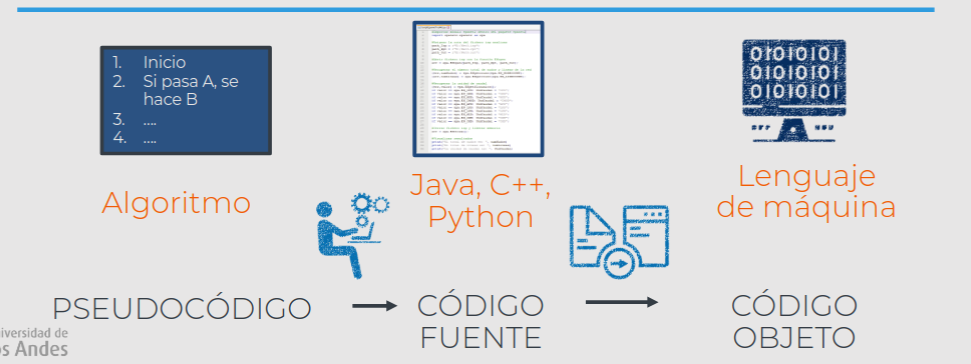
\includegraphics[width=1\linewidth]{Algoritmos.png}
    \caption{Algoritmos}
    \label{fig:enter-label}
\end{figure}
\section{Introduccion a la Programacion}
Las computadoras son simples objetos sin instrucciones las cuales pueda ejecutar. De ahi nace la palabra de algoritmo. Un \textbf{algoritmo} es una secuencia de pasos a desarrollar para cumplir un objetivo en concreto y esto traducido a un lenguaje la cual la maquina pueda entender, se conoce como \textbf{programa}. El lenguaje es el medio y la herramienta de comunicacion y expresion mas conocida en nuestro mundo, por ende: \\
Existen dos tipos de lenguajes:
\begin{itemize}
    \item Natural: Aquel que los seres humanos desarrollamos (Corporal, palabras, etc)
    \item Programacion: Son los lenguajes de maquina, es decir, el lenguaje que usa la maquina para ejecutar los algoritmos. Sin embargo, este es diseñado por humanos y no por las maquinas.
\end{itemize}
Los lenguajes poseen 4 grandes componentes:
\begin{enumerate}
    \item Un alfabeto: Conjunto de simbolos para formar palabras (Ingles, Ruso, Japones).
    \item Lexico: Conjunto de palabras que el lenguaje ofrece a sus usuarios. 
    \item Sintaxis: Conjunto de reglas que hacen que las posibles combinaciones de palabras tengan sentido.
    \item Semantica: Lo mismo que la sintaxis solo que con frases enteras.
\end{enumerate}
Debido a la necesidad de que los humanos nos comunicaramos con las maquinas, surgen una mezcla de lenguajes intermedios que:
\begin{itemize}
    \item No son tan simples como el lenguaje de maquina
    \item No son tan complejos como el lenguaje natural
\end{itemize}
Surgen los \textbf{Lenguajes de Programacion de alto nivel}, los cuales permiten a los humanos dar instrucciones a las maquinas por medio de una combinacion de simbolos nueva que los humanos puedan entender. Estos tambien se conocen como \textbf{codigos fuente} y se guardan en \textbf{archivos fuente}.
\subsection{Compilacion vs Interpretacion}
Es el principio de convertir el codigo fuente en lenguaje de maquina para que la computadora pueda desarrollar cada una de las instrucciones descritas en dicho codigo. Ahora bien, este proceso afortunadamente lo realiza la computadora para que sea mas rapido y efeciente. 
\subsubsection{Compilacion}
El codigo fuente se traduce una vez generando un archivo ejecutable o \textit{.exe} con el cual se puede ejecutar el programa realizado. Sin embargo, cada vez que se genere un cambio en el codigo fuente, este proceso se tiene que repetir una y otra vez. Quien realiza esta accion se denomina \textbf{compilador} o \textbf{traductor}. 
\subsubsection{Interpretacion}
Cualquier persona puede traducir el codigo cada vez que este se deba ejecutar, ya que la funcion de un \textbf{interprete} es interepretar el codigo cada vez que se ejecute. Sin embargo, el codigo no se puede distribuir libremente sin asegurarse que las otras personas tengan el interprete instalado en su sistema. Un iterprete realiza los siguentes pasos:
\begin{enumerate}
    \item Lee el codigo de arriba a abajo y de derecha a izquierda
    \item Verifica los 4 componentes del lenguaje
    \item Si encuentra un error, finaliza la tarea dando la informacion de ese error al usuario
    \item Termina ejecucion (Exito o Fracaso)
\end{enumerate}
\begin{figure}[H]
    \centering
    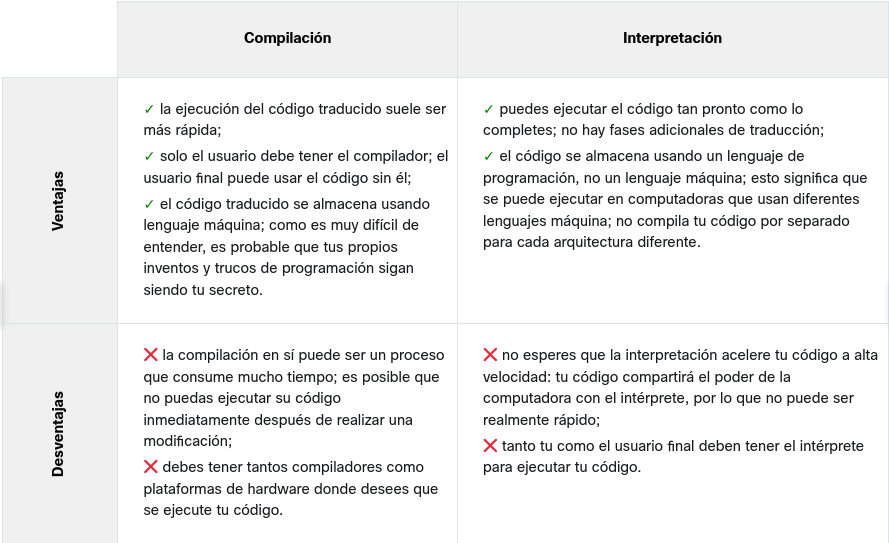
\includegraphics[width=0.75\linewidth]{CompiladorvsInterprete.png}
    \caption{Ventajas y Desventajas de ambos modelos}
    \label{fig:enter-label}
\end{figure}
A todo esto, es para que sepas que \textbf{Python} es un Lenguaje interpretado, es decir, utiliza el modelo del interprete y sus caracteristicas, ademas a este tipo de lenguajes de interprete se les conoce como \textbf{Lenguajes de Scripting}.
\section{Python}
Python es un lenguaje de programacion de alto nivel, interpretado y OOP con un uso generalizado con semantica dinamica. La seleccion de python se da poe los siguentes aspectos:
\begin{itemize}
    \item Facil de aprender: Su tiempo de aprendizaje es mas corto que otros lenguajes de programacion.
    \item Facil de enseñar: No requiere de trucos exoticos, cosas xtrañas o cosas por el estilo, tan solo requiere tecnicas generales de programacion.
    \item Facil de utilizar: CCuando se implemneta software es mas facil hacerlo en python.
    \item Facil de entender: Ya que se asumeja mucho al ingles.
\end{itemize}
\subsection{Competidores}
\begin{enumerate}
    \item Perl: Derivado de C
    \item Ruby: Mas creativo
\end{enumerate}
Python se encuentra entre estos dos tipos de lenguajes, respetando lo clasico pero a su vez siendo innovador. 
\subsection{Usos}
Este se encuentra en una gran cantidad de aplicaciones, desde servidores de internet, almacenamiento en nube, redes sociales, etc. Sin embago, python no llega a todas las areas, unas de estas son:
\begin{itemize}
    \item Programacion alto nivel:  Aca el ideal o el rey es C
    \item Aplicaciones moviles
\end{itemize}
\subsection{Tipos}
Existen dos tipos de python: 
\begin{itemize}
    \item Python 2: Es un tipo estancado, con actualizaciones centradas en corregir errores mas no revolucionar el lenguaje.
    \item Python 3: La version mas actual y versatil de python
\end{itemize}
Estas dos versiones son incompatibles entre si. Ademas cabe resaltar que ambas versiones estas implementadas en C.
\subsection{Mensajes de error}
Estos se componen  de 4 partes: 
\begin{itemize}
    \item TraceBack: La ruta que recorre el codigo al momento de la ejecucion.
    \item Ubicacion del error: Es el nombre del archivo, la linea y el nombre del modulo (Es engañoso ya que es cuando python detecta por primera vez el error, mas no significa que sea ahi). 
    \item Nombre del error y explicacion de este.
\end{itemize}
\section{Valores y Tipos de Datos}
Los valores son aquellos los cuales son manipulados por los programas para hacer tareas especificas. Estos se pueden clasificar de acuerdo a su tipo:
\begin{itemize}
    \item Enteros - \textbf{int}: Ocupan menos memoria y son mas rapidas sus operaciones.
    \item Decimales - \textbf{float}
    \item Strings o texto - \textbf{str}: Cadena o secuencia de caracteres de cualquier cosa.
\end{itemize}
Para conocer el tipo de valor que estas manejando, \textbf{python} tiene una funcion predefinida llamada \textit{type} la cual indica que tipo de dato es un valor. 
\subsection{Enteros}
Son aquellos numeros que no tienen partes fraccionarias. Hay distintos tipos de numeros en python:
\begin{itemize}
    \item Binario: 0,1
    \item Octal:0oNumero
    \item Hexadecimal: 0xNumero
    \item \(\mathbb{N}\): Los naturales (Positivos y Negativos)
\end{itemize}
\subsection{Flotantes}
Son aquellos numeros los cuales si poseen parte decimal o fraccionaria. 
\begin{itemize}
    \item Fraccionarios: \(\frac{Numero}{Numero}\) o \(Numero.Numero\)
    \item Notacion cientifica: Python permite el uso de \textit{e} como la notacion cientifica de \(10^N\)
\end{itemize}
\subsection{Cadenas}
Son el conjunto de caracteres de texto encerrados entre las comillas dobles o sencillas.
\subsection{Booleanos}
Son el True y el False o 1 y 0. Estos estan mejor definidos en al algebra booleana (Revisar Introduccion a la programacion)
\section{Variables e instrucciones de asignacion}
Las \textbf{variables} son una parte fundamental de un programa, estas en pocas palabras son \textit{contenedores} en los cuales se pueden \textbf{almacenar} valores de distintos tipos, con el fin de usarlas mas adelante en el programa. Ahora bien, La instruccion de \textbf{asigancion} es aquella que permite guardar los valores en las variables y se representa por medio de un \(=\). Ademas, hay que tener en cuenta que las varibales solo recuerdan el ultimo valor asignado, por ende, si se cambia, no se podra recuperar. \\
Por otra parte, una caracteristica interesante de \textbf{python} es su \textit{tipado dinamico}, es decir, una variable puede cambiar entre tipos de datos, de int a str o float y viceversa.\\
Retomando lo anterior, las variables son reconocidas por su nombre, el cual actua como un \textbf{identificador} unico de cada variable. Sin embargo, estas tienen restricciones: 
\begin{enumerate}
    \item Pueden contener: letras, digitos, caracteres especiales
    \item Los identificadores no pueden iniciar con un digito
    \item Se distingue entre mayusculas y minusculas
    \item No pueden coincidir con palabras reservadas
\end{enumerate}
\begin{figure}[H]
    \centering
    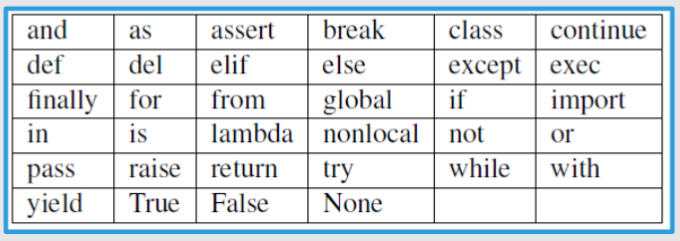
\includegraphics[width=1\linewidth]{PalabrasReservadas.png}
    \caption{Palabras Reservadas Python}
    \label{fig:enter-label}
\end{figure}
\subsection{Expresiones y Operadores}
Las expresiones, son una combinacion entre las \textbf{variables}, \textbf{operadores} y \textbf{valores}. Estas expresiones se desarrollan con el fin de obtener un \textbf{valor} en concreto ya que su finalidad es ser almacenadas en variables para ser usadas mas adelante.
\subsubsection{Operadores y Operandos aritmeticos}
Los operadores son simbolos los cuales representan instrucciones o calculos como las operaciones aritmeticas.
\begin{figure}[H]
    \centering
    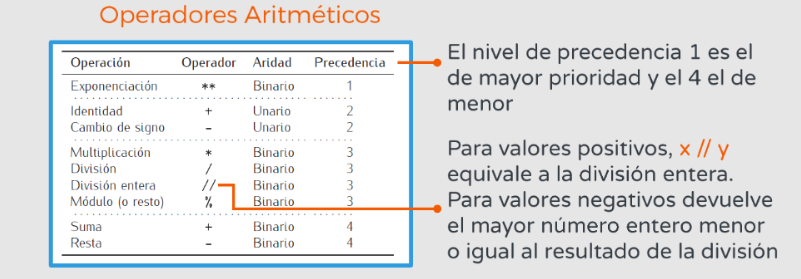
\includegraphics[width=1\linewidth]{OperadoresAritmeticos.png}
    \caption{Operadores Aritmeticos}
    \label{fig:enter-label}
\end{figure}
\subsubsection{Operadores Strings}
Dentro de los operadores, no solo existen operaciones sobre numeros (int, float) sino que tambien existen sobre los \textbf{strings}:
\begin{itemize}
    \item \textbf{Suma (+)}: Este operador no actua como en numeros, sino que en este caso su funcion es \textbf{concatenar} o \textbf{pegar} dos strings.
    \item \textbf{Multiplicacion (*)}: Este operador cumple la funcion de \textbf{repeticion}, es decir, repite un string \(n\) veces el cual es el numero por el cual se repetira el string.
\end{itemize}
\begin{lstlisting}[language=Python, caption=Operaciones sobre Strings]
SumaStrings = "Hola " + "Como estas?"
MultiplicacionStrings = "Hola"*5
\end{lstlisting}
El resultado de esto sera:
\begin{lstlisting}[language=Python, caption=Operaciones sobre Strings]
Hola Como estas?
HolaHolaHolaHolaHola
\end{lstlisting}
\subsection{Conversion de tipos}
Los tipos de dato pueden ser convertidos de unos a otros, esto en python se hace por medio de las funciones:
\begin{enumerate}
    \item int(): La cual convierte strings numericos("123") y floats a numeros enteros. 
    \item float(): La cual convierte strings flotantes("12.3") y ints a numeros flotantes o decimales.  
    \item str(): La cual convierte ints y floats a strings o cadenas de texto. 
\end{enumerate}
\section{Programas}
\subsection{Funciones}
Hasta el momento se han usado funciones basicas de python como lo son:
\begin{enumerate}
    \item str()
    \item int()
    \item float()
    \item type()
\end{enumerate}
Estas ya son funciones predefinidas por el lenguaje, sin embargo hay muchisimas funciones mas.
\begin{itemize}
    \item abs(): Valor absoluto.
    \item round(): Redondeo numeros a \(n\) decimales o a enteros.
    \item min(): Numero minimo.
    \item max(): Numero maximo.
    \item pow(): Elevar un numero a la potencia de \(n\).
\end{itemize}
Asi mismo, como existen funciones numericas como ya las antes mencionadas, existen funciones sobre las cadenas de caracteres.
\begin{itemize}
    \item ord(): Devuelve el valor numerico de un caracter en la tabla ASCII.
    \item chr(): Dado un valor numerico devuelve el caracter asociado segun ASCII.
\end{itemize}
Ahora bien, las funciones van mas alla de los tipos de dato, como por ejemplo.
\begin{itemize}
    \item input(): Funcion de entrada que permite leer datos tecleados por el usuario (Consola).
    \item print(): Imprimir algo en pantalla (Consola).
    \item help(): Es una funcion dada otra funcion, nos explica que hace la funcion pasada como parametro.
\end{itemize}
Sin embargo, existen un sin fin de funciones que pueden:
\begin{itemize}
    \item Estar integradas con python
    \item Provenir de modulos externos de python
    \item De tu codigo (Definicion de funciones)
\end{itemize}
Algo importante que resaltar sobre las funciones en cualquier lenguaje de programacion, es que cada una de estas debe tener un nombre \textbf{unico} y \textbf{descriptivo} con el fin de que sea mas sencillo conocer o recordar cual es su objetivo.
\subsection{Argumentos}
Estos hacen parte de una funcion, estos son ni mas ni menos, aquel valor o valores que necesita la funcion para producir un efecto o resultado, pueden existir funciones sin argumentos, sin embargo, es muy inusual considerando que casi todas las acciones requieren tener algo a la mano o un valor en dado caso. 
\begin{lstlisting}[language=Python, caption=Tu primer Programa]
print("Hola, Mundo!")
\end{lstlisting}
Aca el argumento es: "Hola, Mundo!". Tambien cabe resaltar que las funciones simpre deben tener parentesis de inicio y cierre con el fin de encerrar los argumentos. 
\subsection{Invocacion}
Este termino se refiere a ni mas ni menos que usar la funcion. Una funcion puede estar definida o puede ser parte del lenguaje pero para usarla, esta debe ser invocada, es decir, se debe escribir el nombre de la funcion ya definda con los argumentos que necesita. 
\subsection{Funcion Print}
Un ejemplo de todo lo dicho anterior es la funcion print, que ademas tiene estos usos interesantes:
\begin{itemize}
    \item Sin parametros: Es un salto de linea.
    \item \(\backslash n\): Es un salto de linea inducido en el parametro.
    \item Las comas: Se usa para separar varios argumentos de la funcion.
    \item end = : Se refiere a con que debe termianr la impresion de los argumentos de la funcion, por default es \(\backslash n\).
    \item sep = : Se refiere a como se deben separar los datos en la impresion.
\end{itemize}
\subsection{Definicion de funciones}
A parte de las funciones predefinidas por el lenguaje de programacion, el programador puede definir o crear nuevas funciones con el fin de enseñarle al lenguaje nuevas carateristicas que antes no era posible hacer.
\begin{lstlisting}[language=Python, caption=Ejemplos de funciones]
def monedas(total):
    nikel = 5
    dime = 10
    total = total*100
    if(total%dime == 0):
        return total/dime
    else:
        numDimes = total//dime
        temp = total - (dime*numDimes)
        numNikel = temp//nikel
        return numDimes + numNikel

def rotar(x1,x2,x3):
    temp = x2
    x2 = x1
    x1 = x3
    x3 = temp  
    return x1,x2,x3

def intereses():
    pesos = float(input('Ingrese su cantidad a invertir: '))
    i = float(input('Ingrese la tasa de interes a invertir: '))
    n = int(input('Ingrese numero de peridodos de la inversion: '))
    return round(pesos*(pow(1+(i/100),n)),2)
\end{lstlisting}
Como se puede observar en los ejemplos, las funciones pueden ser \textbf{invocadas}, es decir, se pueden usar, pero tambien las componen ciertas partes. 
\begin{itemize}
    \item Signatura def: Es lo que se usa para definir una funcion. 
    \item Nombre de la func ion: Nombre caracteristico que la diferencia del resto y va despues de la signatura \textit{def}.
    \item Parametros o valores de entrada: Son los que van en los parentesis.
    \item Cuerpo de la funcion: Son todas las instrucciones necesarias a hacer para la funcion.
    \item Instruccion de retorno: el lo ultimo de la funcion, y tiene el papel de dar al usuario el resultado de la funcion dados unos parametros.
\end{itemize}
Cabe resaltar que: 
\begin{enumerate}
    \item Las funciones son independientes y diferentes
    \item Un \textbf{argumento} es lo que se le pasa a la funcion cuando se \textbf{invoca} y un \textbf{parametro} es el que \textbf{hace parte de la funcion} y es necesario para el funcionamiento. 
    \item Cuando se piden mas de 2 valores a una funcion, es mala practica usar la funcion input con el fin de obtenerlos del teclado, por ende, deben ser parametros.
    \item En las funciones, hay un tipo de variables llamadas \textbf{variables locales}, estas son aquellas que solo son usadas en una funcion y nadie mas las puede usar. 
\end{enumerate}
\section{Estilo de programacion}
Se recomienda hacer lo siguente cuando se programa:
\begin{enumerate}
    \item Nombres de varibles y funciones distintivos
    \item Documentacion de funciones: Descripcion, Parametros y Retorno
    \item Siempre intentar usar instrucciones sencillas
    \item Descomposicion de funciones, una funcion cumple una sola actividad
    \item Comentarios de instrucciones
\end{enumerate}
\section{Modulos}
Son colecciones de funciones y de valores que se encuentran en un archivo. Estos se pueden usar en diferentes programas con el fin de no tener que programar las instrucciones una y otra vez.\\
Finalmente, para hacer uso de estos conjuntos de funciones, se usa la palabra \textit{import}. 
\section{Interfaz Usuario}
Los programas deben ser:
\begin{itemize}
    \item Seguros
    \item Buen desempeño
    \item facil de usar (Usabilidad)
    \item Escalable
    \item Tolerante a fallos
    \item Tolerable a cambios (Mantenibilidad)
\end{itemize}
La interfaz de usaurio es la forma de comunicacion entre el usuario y el programa desarrollado. Esta debe ser un modulo separado de la logica del programa, es decir no pueden estar en el mismo archivo. Ademas, asi como existe la funcion \textbf{print} con el fin de presentarle al usuario los resultados de algunas operaciones, tambien existen funciones que permiten al usuario interactuar directamente con el. La funcion mas conocida para la interaccion con el usuario por medio de consola es la funcion \textbf{input()}.  
\end{document}
